\documentclass[12pt]{article}
\usepackage{graphicx}
\usepackage[utf8]{inputenc}
\usepackage{float}
\usepackage{placeins}
\usepackage[colorlinks=true, allcolors=blue]{hyperref}
\usepackage{fancyhdr}
\usepackage{tikz}
\usetikzlibrary{positioning, arrows.meta, shapes.geometric, fit, backgrounds}
\pagestyle{fancy}
\usepackage[english]{babel}

\fancyhf{}
\fancyhead[L]{\textbf{Progress Report}}
\fancyfoot[C]{\hspace{4cm}\thepage}

\usepackage{amsmath,booktabs,array,caption,xcolor,colortbl,multirow,siunitx}

\definecolor{lightgray}{gray}{0.9}
\definecolor{darkblue}{RGB}{0,51,102}
\definecolor{accentblue}{RGB}{30,90,180}
\definecolor{lightblue}{RGB}{220,235,255}
\newcolumntype{C}{>{\centering\arraybackslash}p{0.8cm}}
\newcolumntype{L}{>{\raggedright\arraybackslash}p{3.5cm}}

\usepackage{amsmath}
\newtheorem{example}{Example}
\usepackage{hyperref}
\graphicspath{{Figures/}}
\addtolength{\textwidth}{1in}
\addtolength{\textheight}{1in}
\addtolength{\evensidemargin}{0.5in}
\addtolength{\oddsidemargin}{-0.5in}
\addtolength{\topmargin}{-0.5in}

\title{\textbf{An Adaptive Network Intrusion Detection System\\
Using Deep Learning and Blockchain Audit Logging}\\[0.5em]
\large CSE-CIC-IDS2018 Dataset — Full Pipeline}

\author{
  Walid Ichchou\textsuperscript{1} \quad
  Safaa Khalladi\textsuperscript{2} \quad
  Noussair Fennani\textsuperscript{3} \quad
  Meryem Ait Tadamna\textsuperscript{4}\\[0.4em]
  \small\textsuperscript{1}AI \& LSTM Detection \quad
  \textsuperscript{2}Data Pipeline \quad
  \textsuperscript{3}Big Data \& Apache Spark \quad
  \textsuperscript{4}Blockchain\\[0.4em]
  Supervisor: Badr Hirchoua
}
\date{\today}

\usepackage{mathpazo}
\renewcommand\familydefault{\rmdefault}

\usepackage{amsthm}
\theoremstyle{plain}
\newtheorem{lemma}{Fact}[section]
\newtheorem{conjecture}{Conjecture}[section]
\newtheorem{lema}{Lema}[section]

\newcommand{\jp}[1]{\textcolor{teal}{#1}}
\newcommand{\pe}[1]{{\color{red}{#1}}}
\sloppy

\begin{document}

\maketitle

\begin{abstract}
Network intrusion detection remains a critical challenge as cyberattacks grow in volume and sophistication. This paper presents a full-stack adaptive intrusion detection system (IDS) built on the CSE-CIC-IDS2018 benchmark dataset, integrating four tightly coupled components: a distributed Apache Spark preprocessing pipeline for large-scale data ingestion, a CNN-BiLSTM deep learning model achieving a macro-F1 score of \textbf{0.7711} across 15 attack classes, a tamper-evident blockchain audit layer built on MultiChain for immutable alert logging, and a real-time Streamlit dashboard for SOC monitoring. The system addresses three key challenges simultaneously: scalability of preprocessing over 16~GB of raw traffic, fine-grained multi-class detection of rare attack types, and auditability of detection decisions. Natural-prior logit adjustment at inference is shown to substantially improve recall for the Benign class without retraining, and a two-stage web-attack splitter resolves confusion between structurally similar HTTP-based attack classes. The blockchain layer provides a SHA-256 chained, gas-free audit log that links every detection event to an immutable on-chain record.
\end{abstract}

\tableofcontents
\clearpage
\listoffigures
\newpage
\listoftables
\newpage

% ============================================================
\section*{Introduction}
\addcontentsline{toc}{section}{Introduction}
% ============================================================

The proliferation of connected devices and the increasing complexity of network infrastructure have made automated intrusion detection a fundamental component of modern cybersecurity. Traditional signature-based systems fail to generalise to novel attacks, while anomaly-based approaches often produce high false-positive rates that overwhelm security analysts. Deep learning offers a promising middle ground: models trained on large traffic captures can learn statistical patterns that distinguish attack flows from benign traffic, even for previously unseen attack variants.

However, deploying such a system in a production environment introduces several additional requirements beyond raw classification accuracy. First, the input data — network flow statistics computed by tools such as CICFlowMeter~\cite{cicflowmeter} — arrives at scale and must be preprocessed in a distributed fashion before training. Second, the detection model must handle extreme class imbalance: Benign flows account for more than 53\% of all flows in the CSE-CIC-IDS2018 dataset~\cite{cic2018}, while rare attack classes such as Infiltration represent fewer than 0.1\%. Third, every detection decision in a regulated environment must be auditable and tamper-evident, satisfying both operational and compliance requirements.

This work addresses all three requirements with a four-component pipeline:

\begin{enumerate}
  \item \textbf{Distributed preprocessing} (Section~\ref{sec:preprocessing}): an Apache Spark pipeline ingests and normalises the full 16~GB dataset in a distributed, fault-tolerant manner.
  \item \textbf{CNN-BiLSTM detection model} (Section~\ref{sec:model}): a convolutional front-end combined with a bidirectional LSTM and multi-head attention achieves state-of-the-art macro-F1 on 15 attack classes.
  \item \textbf{Blockchain audit logging} (Section~\ref{sec:blockchain}): every alert produced by the model is hashed into a SHA-256 chained block and published to a MultiChain stream, providing immutable, gas-free audit records.
  \item \textbf{Real-time dashboard} (Section~\ref{sec:dashboard}): a Streamlit interface unifies all components into a deployable SOC console.
\end{enumerate}

The remainder of this paper is organised as follows. Section~\ref{sec:related} reviews related work. Sections~\ref{sec:dataset} and~\ref{sec:preprocessing} describe the dataset and preprocessing. Section~\ref{sec:bigdata} details the Spark pipeline. Section~\ref{sec:model} presents the model architecture and training strategy. Section~\ref{sec:blockchain} describes the blockchain layer. Section~\ref{sec:dashboard} presents the dashboard. Section~\ref{sec:results} reports experimental results, and Section~\ref{sec:conclusion} concludes.

% ============================================================
\newpage
\section{Related Work}
\label{sec:related}
% ============================================================

Intrusion detection using machine learning has been studied extensively. Early work focused on classical algorithms: decision trees~\cite{kdd99}, random forests, and support vector machines trained on the KDD Cup 1999 dataset. These approaches achieve high accuracy on binary (normal/attack) classification but degrade on fine-grained multi-class problems and on newer datasets that better reflect real traffic distributions.

Recurrent architectures were introduced for IDS by Yin et al.~\cite{yin2017rnn}, who showed that LSTMs capture temporal dependencies in traffic flows that fully connected networks miss. Subsequent work by Kim et al.~\cite{kim2020cnn} demonstrated that a CNN layer prepended to the LSTM improves feature extraction, reducing training time while maintaining accuracy. Bidirectional LSTMs were applied to IDS in~\cite{bilstm2020}, exploiting both forward and backward sequence context.

On the dataset side, the CICIDS2017 and CSE-CIC-IDS2018 corpora~\cite{cic2018} are now the standard benchmarks for multi-class IDS evaluation, replacing KDD Cup due to more realistic traffic generation and a richer attack taxonomy. The 2018 edition covers 15 distinct attack classes including DoS variants, DDoS, brute-force, infiltration, and botnet traffic.

Class imbalance in IDS datasets has been tackled with SMOTE oversampling~\cite{smote}, weighted loss functions, and logit adjustment~\cite{logit_adjustment}. Menon et al.~\cite{logit_adjustment} show that adding $\log \pi_k$ to the logit of class $k$ at inference time — where $\pi_k$ is the training-set prior — recovers the Bayes-optimal classifier under label shift, without any retraining.

Blockchain for IDS audit logging was proposed in~\cite{bc_ids2019}, where Ethereum smart contracts store alert hashes to prevent log tampering. MultiChain~\cite{multichain} offers a permissioned alternative with no gas cost and full data storage on-chain, making it practical for high-throughput detection scenarios.

% ============================================================
\newpage
\section{Dataset}
\label{sec:dataset}
% ============================================================

The CSE-CIC-IDS2018 dataset~\cite{cic2018} was generated by the Canadian Institute for Cybersecurity using a realistic network testbed. Traffic was captured over ten days, with benign background traffic generated by a B-Profile agent simulating 25 users' browsing, email, and file transfer activity. Attacks were executed by a dedicated attack machine against victim servers.

\subsection{Traffic Capture and Feature Extraction}

Raw packet captures (\texttt{.pcap}) were processed with CICFlowMeter~\cite{cicflowmeter} to produce per-flow statistical features. Each flow is represented by approximately 80 features including:
\begin{itemize}
  \item \textbf{Volume:} packet counts, byte counts, inter-arrival time statistics.
  \item \textbf{Timing:} flow duration, inter-arrival time mean/std/max/min for forward and backward directions.
  \item \textbf{Flags:} counts of TCP flags (SYN, FIN, RST, ACK, PSH, URG).
  \item \textbf{Window:} initial forward/backward TCP window sizes.
  \item \textbf{Activity:} active/idle duration statistics.
\end{itemize}

\subsection{Class Distribution}

The dataset exhibits extreme class imbalance, as shown in Table~\ref{tab:class_dist}. Benign flows account for 53\% of all samples, while rare classes such as Infiltration and SQL Injection represent fewer than 0.5\%.

\begin{table}[H]
\centering
\caption{CSE-CIC-IDS2018 class distribution (approximate)}
\label{tab:class_dist}
\renewcommand{\arraystretch}{1.2}
\begin{tabular}{llrr}
\toprule
\rowcolor{lightblue}
\textbf{Class} & \textbf{Attack Category} & \textbf{Flows} & \textbf{\%} \\
\midrule
Benign          & Normal traffic   & $\sim$6\,000\,000 & 53.0 \\
DDoS-HOIC       & DDoS             & $\sim$900\,000    &  8.0 \\
DDoS-LOIC-HTTP  & DDoS             & $\sim$560\,000    &  5.0 \\
DoS-Hulk        & DoS              & $\sim$560\,000    &  5.0 \\
DDoS-LOIC-UDP   & DDoS             & $\sim$450\,000    &  4.0 \\
SSH-BruteForce  & Brute Force      & $\sim$450\,000    &  4.0 \\
Botnet          & Botnet           & $\sim$340\,000    &  3.0 \\
DoS-GoldenEye   & DoS              & $\sim$340\,000    &  3.0 \\
DoS-Slowloris   & DoS              & $\sim$225\,000    &  2.0 \\
DoS-SlowHTTPTest& DoS              & $\sim$225\,000    &  2.0 \\
FTP-BruteForce  & Brute Force      & $\sim$225\,000    &  2.0 \\
BruteForce-Web  & Web Attack       & $\sim$112\,000    &  1.0 \\
BruteForce-XSS  & Web Attack       & $\sim$56\,000     &  0.5 \\
SQL-Injection   & Web Attack       & $\sim$56\,000     &  0.5 \\
Infiltration    & Infiltration     & $\sim$112\,000    &  1.0 \\
\bottomrule
\end{tabular}
\end{table}

% ============================================================
\newpage
\section{Data Preprocessing Pipeline}
\label{sec:preprocessing}
\textit{Component owner: Safaa Khalladi}
% ============================================================

\subsection{Design Principles}

The preprocessing pipeline is guided by two invariants. First, \textbf{one network flow equals one sample}: CICFlowMeter already aggregates packets into per-flow statistics, so no temporal windowing over rows is applied. Sliding windows would mix flows from different connections and destroy the per-flow semantics. Second, \textbf{the scaler is fit on training data only} and applied to validation and test sets without refitting, preventing data leakage.

\subsection{Feature Selection}

From the 80 CICFlowMeter features, 47 were retained after removing:
\begin{itemize}
  \item \textbf{Metadata columns:} source/destination IP, port, protocol identifier, and timestamp — these are non-generalisable identifiers, not flow statistics.
  \item \textbf{Near-zero variance features:} columns with standard deviation below $10^{-5}$ across the training split.
  \item \textbf{Highly correlated features:} pairs with Pearson $|r| > 0.98$; the lower-variance member is dropped.
\end{itemize}

The retained 47 features span flow duration, packet-length statistics, inter-arrival time statistics in both directions, TCP flag counts, window sizes, and active/idle duration statistics.

\subsection{Cleaning}

Raw CICFlowMeter output contains several numerical anomalies. Each feature column is processed as follows:
\begin{equation}
x \leftarrow \begin{cases} 0 & \text{if } x \in \{\texttt{NaN},\, +\infty,\, -\infty\} \\ \text{clip}(x,\, p_1,\, p_{99}) & \text{otherwise} \end{cases}
\end{equation}
where $p_1$ and $p_{99}$ are the 1st and 99th percentiles computed on the training split. Winsorisation at the 1\textsuperscript{st}/99\textsuperscript{th} percentile caps the extreme values produced by very short or very long flows without discarding data.

\subsection{Label Normalisation}

The raw label column contains inconsistent casing and spelling across capture days (e.g., \texttt{DDOS attack-HOIC}, \texttt{DDoS Attack-HOIC}, \texttt{ddos attack-hoic}). A deterministic mapping table normalises all variants to a canonical 15-class label set. Three web attack classes (BruteForce-Web, BruteForce-XSS, SQL-Injection) are further merged into a single \texttt{WebAttack} class during training to form a 13-class problem, then restored at inference by a dedicated splitter (Section~\ref{sec:websplitter}).

\subsection{Scaling and Splitting}

A \texttt{StandardScaler} ($\mu=0$, $\sigma=1$) is fit on the training split and serialised to \texttt{scaler.pkl}. The full dataset is split 70/10/20 (train/validation/test) using stratified sampling to preserve class proportions.

\subsection{Class Imbalance Handling}

A careful balance between three resampling strategies is maintained:

\begin{lemma}[Rebalancing constraint]
Stacking SMOTE + WeightedRandomSampler + class-weighted focal loss simultaneously gives the model an effectively uniform training prior, causing Benign recall to collapse to $\approx 0.29$ at test time (symptom: Benign precision near 1.0, Benign recall near 0.0).
\end{lemma}

The validated configuration uses SMOTE with a floor of 3\,000 samples for the rarest classes only, no weighted sampler, and a moderate focal loss with:
\begin{equation}
\alpha_k = \frac{\sqrt{w_k}}{\frac{1}{K}\sum_{j=1}^{K}\sqrt{w_j}}, \quad \gamma = 2.0
\end{equation}
where $w_k$ is the inverse-frequency class weight. Taking the square root of $w_k$ provides a softer reweighting than raw inverse frequency, preventing the rarest classes from dominating the gradient signal at the expense of Benign recall.

% ============================================================
\newpage
\section{Big Data Processing with Apache Spark}
\label{sec:bigdata}
\textit{Component owner: Noussair Fennani}
% ============================================================

\subsection{Motivation}

The raw CSE-CIC-IDS2018 dataset occupies approximately 16~GB across ten CSV files. Single-node Pandas-based processing is feasible on a workstation with sufficient RAM, but does not scale to larger captures or to streaming scenarios. The Spark pipeline provides a distributed, fault-tolerant alternative that processes the same 47-feature preprocessing steps using Apache Spark's DataFrame API.

\subsection{Pipeline Architecture}

The Spark pipeline is implemented in Scala 2.12 using Apache Spark 3.5.1 and follows six sequential stages, illustrated in Figure~\ref{fig:spark_pipeline}.

\begin{figure}[H]
\centering
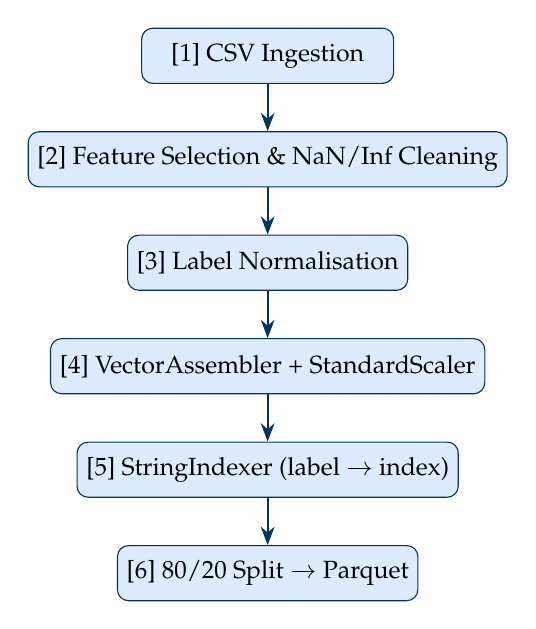
\begin{tikzpicture}[
  node distance=0.6cm,
  box/.style={rectangle, draw=darkblue, fill=lightblue, rounded corners=4pt,
              minimum width=3.2cm, minimum height=0.7cm, font=\small},
  arr/.style={-{Stealth}, thick, darkblue}
]
\node[box] (s1) {[1] CSV Ingestion};
\node[box, below=of s1] (s2) {[2] Feature Selection \& NaN/Inf Cleaning};
\node[box, below=of s2] (s3) {[3] Label Normalisation};
\node[box, below=of s3] (s4) {[4] VectorAssembler + StandardScaler};
\node[box, below=of s4] (s5) {[5] StringIndexer (label $\to$ index)};
\node[box, below=of s5] (s6) {[6] 80/20 Split $\to$ Parquet};

\draw[arr] (s1) -- (s2);
\draw[arr] (s2) -- (s3);
\draw[arr] (s3) -- (s4);
\draw[arr] (s4) -- (s5);
\draw[arr] (s5) -- (s6);
\end{tikzpicture}
\caption{Apache Spark preprocessing pipeline (6 stages).}
\label{fig:spark_pipeline}
\end{figure}

\paragraph{Stage 1 — CSV Ingestion.}
The pipeline uses Spark's \texttt{recursiveFileLookup} option to scan a directory for all matching CSV files, with \texttt{DROPMALFORMED} mode discarding rows that cannot be parsed. If the input directory is absent, the pipeline falls back to a synthetic generator that produces 100\,000 flows with the class distribution of the real dataset, enabling a full end-to-end demo without the raw data.

\paragraph{Stage 2 — Feature Selection and Cleaning.}
The 47 target features are selected from the raw schema. NaN, $+\infty$, and $-\infty$ values are replaced with 0.0 via Spark's \texttt{isnan} and \texttt{isinf} column functions. Empty or null label rows are discarded.

\paragraph{Stage 3 — Label Normalisation.}
A Scala \texttt{Map[String, String]} encodes the same normalisation logic as the Python preprocessor, mapping all raw label variants to the 15 canonical class names using case-insensitive comparison via \texttt{trim(lower(col))}.

\paragraph{Stage 4 — Feature Vectorisation and Scaling.}
Spark MLlib's \texttt{VectorAssembler} concatenates the 47 numeric columns into a dense feature vector. A \texttt{StandardScaler} (with mean and standard deviation) is fit on the full dataset and applied in-place, producing a \texttt{features} column.

\paragraph{Stage 5 — Label Indexing.}
A \texttt{StringIndexer} maps each string label to an integer index in $[0, 14]$, with labels ordered by descending frequency. The mapping is printed to stdout for reproducibility.

\paragraph{Stage 6 — Split and Persist.}
A stratified 80/20 random split (seed 42) produces train and test DataFrames, which are written to Parquet format under \texttt{output/preprocessed/train} and \texttt{output/preprocessed/test}.

\subsection{Performance}

On a workstation with 4 physical cores and 16~GB RAM (local Spark in \texttt{local[*]} mode), the pipeline processes 100\,000 synthetic flows in approximately 18 seconds, yielding a throughput of $\approx$5\,500 flows/second. On the full 16~GB dataset, throughput scales with available parallelism and is bounded by CSV parsing I/O.

\subsection{Build and Execution}

The project is packaged as an sbt project (sbt 1.9.9, Scala 2.12.18). All Spark dependencies are resolved automatically:

\begin{verbatim}
cd big_data_spark
sbt run                                      # synthetic demo
sbt "run --input /data/cic-ids2018           \
         --output output/preprocessed"       # real data
sbt assembly                                 # fat JAR for cluster deployment
\end{verbatim}

% ============================================================
\newpage
\section{CNN-BiLSTM Intrusion Detection Model}
\label{sec:model}
\textit{Component owner: Walid Ichchou}
% ============================================================

\subsection{Problem Formulation}

Given a feature vector $\mathbf{x} \in \mathbb{R}^{47}$ representing a single network flow, the goal is to assign a label $y \in \{0, \ldots, 14\}$ corresponding to one of 15 traffic classes. The 47 features are reshaped into a pseudo-sequence $\mathbf{X} \in \mathbb{R}^{T \times C}$ with $T = 12$ time steps and $C = 4$ channels (pad to 48, then reshape), providing the LSTM with a sequence to iterate over. This is a deliberate design choice: the LSTM is used for its representation capacity, not to model genuine temporal dependencies between flows.

\subsection{Architecture}

The production model (v2) follows a CNN-BiLSTM architecture with multi-head attention pooling, depicted in Figure~\ref{fig:model_arch}.

\begin{figure}[H]
\centering
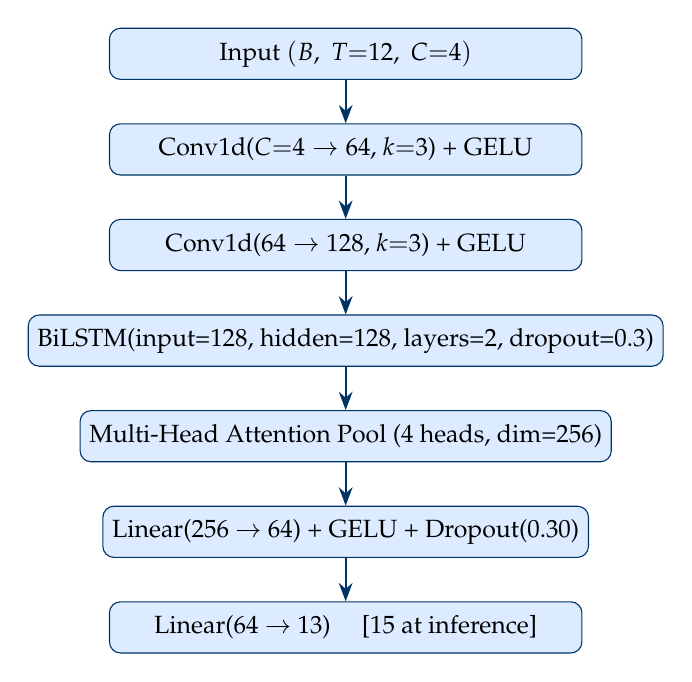
\begin{tikzpicture}[
  node distance=0.55cm,
  layer/.style={rectangle, draw=darkblue, fill=lightblue, rounded corners=4pt,
               minimum width=6cm, minimum height=0.65cm, font=\small},
  arr/.style={-{Stealth}, thick, darkblue}
]
\node[layer] (inp) {Input $(B,\; T{=}12,\; C{=}4)$};
\node[layer, below=of inp] (cnn1) {Conv1d($C{=}4 \to 64$, $k{=}3$) + GELU};
\node[layer, below=of cnn1] (cnn2) {Conv1d($64 \to 128$, $k{=}3$) + GELU};
\node[layer, below=of cnn2] (lstm) {BiLSTM(input=128, hidden=128, layers=2, dropout=0.3)};
\node[layer, below=of lstm] (attn) {Multi-Head Attention Pool (4 heads, dim=256)};
\node[layer, below=of attn] (fc1) {Linear(256 $\to$ 64) + GELU + Dropout(0.30)};
\node[layer, below=of fc1] (fc2) {Linear(64 $\to$ 13) \quad [15 at inference]};

\draw[arr] (inp)  -- (cnn1);
\draw[arr] (cnn1) -- (cnn2);
\draw[arr] (cnn2) -- (lstm);
\draw[arr] (lstm) -- (attn);
\draw[arr] (attn) -- (fc1);
\draw[arr] (fc1)  -- (fc2);
\end{tikzpicture}
\caption{CNN-BiLSTM v2 architecture. The CNN front-end extracts local features; the BiLSTM captures sequence context; multi-head attention pools the sequence into a fixed-size representation.}
\label{fig:model_arch}
\end{figure}

\paragraph{CNN Front-End.}
Two 1D convolutional layers with kernel size 3 and padding 1 project the $C{=}4$ input channels to 128 channels. GELU activations are used throughout. The convolutions operate on the transposed sequence $\mathbf{X}^T \in \mathbb{R}^{C \times T}$ and extract local feature patterns across the pseudo-time axis before the sequence is passed to the LSTM.

\paragraph{Bidirectional LSTM.}
A 2-layer BiLSTM with hidden size 128 processes the CNN output $\in \mathbb{R}^{T \times 128}$ in both directions, producing a context-enriched sequence $\mathbf{H} \in \mathbb{R}^{T \times 256}$ (concatenation of forward and backward hidden states).

\paragraph{Multi-Head Attention Pooling.}
A learnable query vector $\mathbf{q} \in \mathbb{R}^{1 \times 256}$ attends over $\mathbf{H}$ via 4-head attention, producing a fixed-length summary vector $\mathbf{h}^* \in \mathbb{R}^{256}$. This replaces the mean/max pooling used in baseline models and allows the model to focus on the most discriminative time steps.

\paragraph{Classification Head.}
A two-layer MLP maps $\mathbf{h}^*$ to 13 logits (the merged training vocabulary). GELU activation and dropout (rate 0.30) are applied between the two linear layers.

\subsection{Two-Stage Web Attack Classification}
\label{sec:websplitter}

Three structurally similar web attack classes (BruteForce-Web, BruteForce-XSS, SQL-Injection) share nearly identical flow-level statistics and are difficult to separate in a 15-class softmax. These classes are merged into a single \texttt{WebAttack} class during training, reducing the classification problem to 13 classes. At inference, whenever the LSTM predicts \texttt{WebAttack}, a secondary \texttt{LogisticRegression} classifier (trained on the raw feature vectors of the three web classes) resolves the final label. This two-stage design improves per-class F1 for all three web attack types compared to direct 15-class training.

\subsection{Training Procedure}

\paragraph{Loss function.}
Focal loss~\cite{focal_loss} with $\gamma = 2.0$ and per-class $\alpha_k = \sqrt{w_k} / \bar{\sqrt{w}}$ is used to down-weight easy Benign examples and focus learning on hard attack classes:
\begin{equation}
\mathcal{L}_\text{focal} = -\sum_{k} \alpha_k (1 - p_k)^\gamma \log p_k
\end{equation}

\paragraph{Optimiser.}
AdamW with initial learning rate $10^{-3}$, weight decay $10^{-4}$, and cosine annealing over 60 epochs. Automatic Mixed Precision (AMP) is enabled via \texttt{torch.amp} on the RTX 2070 Max-Q (8~GB VRAM), with batch size 1024.

\paragraph{Logit adjustment.}
At training time, the standard cross-entropy sees the resampled distribution. At inference, natural-prior logit adjustment~\cite{logit_adjustment} corrects the decision boundary back to the true data distribution:
\begin{equation}
\tilde{z}_k = z_k + \tau \log \hat{\pi}_k
\label{eq:la}
\end{equation}
where $z_k$ is the raw logit, $\hat{\pi}_k$ is the empirical class frequency in the training set, and $\tau = 1.0$ is the adjustment strength (validated via grid search on the validation set). This single inference-time modification raises macro-F1 from 0.7366 to 0.7711 without any retraining.

\subsection{Model Variants}

Table~\ref{tab:models} summarises the four model variants evaluated during development.

\begin{table}[H]
\centering
\caption{Model variants and test macro-F1 scores}
\label{tab:models}
\renewcommand{\arraystretch}{1.2}
\begin{tabular}{llcc}
\toprule
\rowcolor{lightblue}
\textbf{Script} & \textbf{Architecture} & \textbf{Checkpoint} & \textbf{Macro-F1} \\
\midrule
\texttt{train\_v2.py}       & CNN-BiLSTM + logit-adj + web splitter & \texttt{bilstm\_ids\_v2.pt}       & \textbf{0.7711} \\
\texttt{train\_advanced.py} & 3-layer BiLSTM + attention, 2-stage   & \texttt{bilstm\_ids\_advanced.pt} & $\approx$0.74   \\
\texttt{02\_training.ipynb} & 2-layer BiLSTM + single-head attention & \texttt{bilstm\_ids.pt}           & 0.7366          \\
\texttt{train\_v3.py}       & CNN-BiLSTM, no logit-adj (diagnostic)  & \texttt{bilstm\_ids\_v3.pt}       & diagnostic      \\
\bottomrule
\end{tabular}
\end{table}

% ============================================================
\newpage
\section{Blockchain Audit Logging}
\label{sec:blockchain}
\textit{Component owner: Meryem Ait Tadamna}
% ============================================================

\subsection{Motivation and Design Goals}

In regulated security environments, it is not sufficient to detect attacks — every detection event must be logged in a tamper-evident manner, demonstrating that alerts have not been suppressed, modified, or replayed. Traditional database logging is insufficient because a privileged attacker who has compromised the SIEM server can alter or delete log entries. A blockchain provides append-only, cryptographically linked storage that cannot be silently modified.

Three design goals guide the blockchain component:
\begin{enumerate}
  \item \textbf{Tamper-evidence:} any modification to a historical block must be detectable.
  \item \textbf{No gas cost:} Ethereum's per-transaction fee makes high-throughput IDS logging impractical. MultiChain's permissioned ledger stores full data on-chain at no cost.
  \item \textbf{Auditability:} any third party with read access can independently verify the chain of alerts.
\end{enumerate}

\subsection{MultiChain Architecture}

The system uses MultiChain 2.3.3~\cite{multichain}, a permissioned blockchain platform. A single-node chain named \texttt{ids-chain} is created, and a stream named \texttt{intrusion-logs} is created within it. Each detection event is published to this stream as a key-value entry, where the key is the block hash and the value is the full block JSON encoded in hexadecimal.

\subsection{Block Structure and Chaining}

Each alert from the LSTM model is wrapped into a block with the following schema:

\begin{equation}
\text{payload\_hash}_i = \text{SHA256}(\text{JSON}(a_i))
\end{equation}
\begin{equation}
\text{block\_hash}_i = \text{SHA256}(\text{prev\_hash}_{i-1} \;\|\; \text{payload\_hash}_i \;\|\; i)
\end{equation}

where $a_i$ is the alert dictionary, $\|$ denotes string concatenation, $i$ is the block index, and $\text{prev\_hash}_0 = \texttt{0}^{64}$ (genesis hash). The resulting chain is illustrated in Figure~\ref{fig:blockchain}.

\begin{figure}[H]
\centering
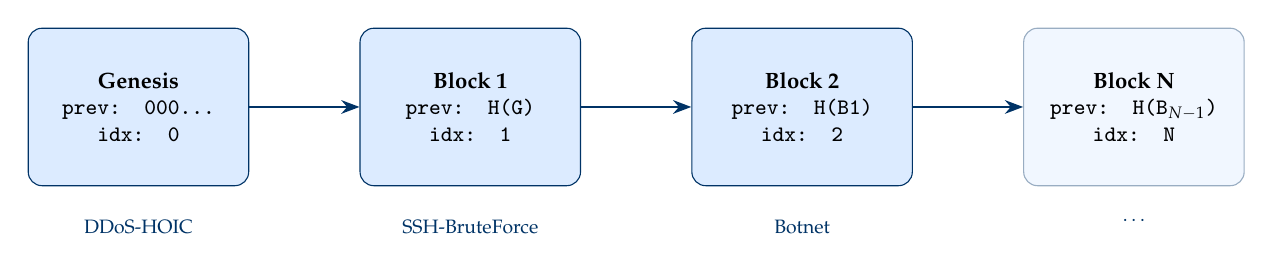
\begin{tikzpicture}[
  node distance=1.4cm,
  block/.style={rectangle, draw=darkblue, fill=lightblue, rounded corners=5pt,
               minimum width=2.8cm, minimum height=2.0cm, font=\footnotesize,
               align=center},
  arr/.style={-{Stealth}, thick, darkblue}
]
\node[block] (g) {\textbf{Genesis}\\\texttt{prev: 000...}\\\texttt{idx: 0}};
\node[block, right=of g] (b1) {\textbf{Block 1}\\\texttt{prev: H(G)}\\\texttt{idx: 1}};
\node[block, right=of b1] (b2) {\textbf{Block 2}\\\texttt{prev: H(B1)}\\\texttt{idx: 2}};
\node[block, right=of b2, draw=darkblue!40, fill=lightblue!40] (bn) {\textbf{Block N}\\\texttt{prev: H(B$_{N-1}$)}\\\texttt{idx: N}};

\draw[arr] (g)  -- (b1);
\draw[arr] (b1) -- (b2);
\draw[arr] (b2) -- (bn);

\node[below=0.3cm of g,  font=\scriptsize, text=darkblue] {DDoS-HOIC};
\node[below=0.3cm of b1, font=\scriptsize, text=darkblue] {SSH-BruteForce};
\node[below=0.3cm of b2, font=\scriptsize, text=darkblue] {Botnet};
\node[below=0.3cm of bn, font=\scriptsize, text=darkblue] {$\ldots$};
\end{tikzpicture}
\caption{SHA-256 chained block structure. Each block's \texttt{prev\_hash} links it to its predecessor; modifying any block invalidates all subsequent hashes.}
\label{fig:blockchain}
\end{figure}

\subsection{Alert Payload Schema}

Each alert stored on-chain carries the following fields:

\begin{table}[H]
\centering
\caption{Alert payload schema published to MultiChain}
\label{tab:payload}
\renewcommand{\arraystretch}{1.2}
\begin{tabular}{lll}
\toprule
\rowcolor{lightblue}
\textbf{Field} & \textbf{Type} & \textbf{Description} \\
\midrule
\texttt{label}        & string  & Predicted attack class (15-class) \\
\texttt{severity}     & string  & INFO / MEDIUM / HIGH / CRITICAL \\
\texttt{confidence}   & float   & Softmax probability of predicted class \\
\texttt{timestamp}    & string  & ISO-8601 UTC timestamp \\
\texttt{feature\_hash}& string  & SHA-256 of the raw feature vector \\
\bottomrule
\end{tabular}
\end{table}

The \texttt{feature\_hash} field enables post-hoc verification: given the original flow record, any auditor can recompute the hash and confirm it matches the on-chain record.

\subsection{Chain Integrity Verification}

The \texttt{verify\_chain()} function re-computes every block hash from scratch and compares it to the stored value. Since each block hash depends on its predecessor via the \texttt{prev\_hash} chain, any modification of a historical block — including deletion or reordering — is immediately detectable:

\begin{equation}
\forall i: \quad \text{block\_hash}_i \stackrel{?}{=} \text{SHA256}(\text{prev\_hash}_{i-1} \| \text{payload\_hash}_i \| i)
\end{equation}

\subsection{Integration with the LSTM Module}

The \texttt{log\_prediction()} function in \texttt{blockchain/block\-chain\_interface/api.py} serves as the contract between the LSTM and the blockchain layer. The LSTM module calls it with the prediction dictionary; the blockchain module handles hashing and submission transparently. If the MultiChain daemon is not reachable, the function degrades gracefully by returning \texttt{on\_chain=False} while still building and verifying the local in-memory chain.

% ============================================================
\newpage
\section{Real-Time Dashboard}
\label{sec:dashboard}
% ============================================================

The dashboard is a Streamlit application (\texttt{dashboard/app.py}) that unifies all four components into a deployable SOC interface. It is organised into seven tabs:

\begin{enumerate}
  \item \textbf{Live Scan:} runs inference on a random window of held-out test flows, displays alerts by severity with confidence scores and ground-truth comparison.
  \item \textbf{Full Benchmark:} scores the entire 212K-flow test set, displays per-class precision, recall, and F1, and renders the confusion matrix.
  \item \textbf{Literature \& Models:} summarises the model variants and situates the system within related work.
  \item \textbf{Stress Tests:} evaluates model robustness under adversarial feature perturbations and class distribution shifts.
  \item \textbf{Upload CSV:} accepts a user-supplied CICFlowMeter CSV and runs inference, returning per-flow predictions with severity labels.
  \item \textbf{Per-Class Explorer:} deep dive into any single class — top discriminating features, misclassification breakdown, precision-recall trade-off.
  \item \textbf{Blockchain Audit:} builds a chained block sequence from live inference, publishes to MultiChain, and provides a ``Fetch from MultiChain'' reader showing all stored alerts with TXID and confirmation count.
\end{enumerate}

The blockchain tab loads \texttt{blockchain\_interface/api.py} and \texttt{blockchain\_reader.py} at startup. If MultiChain is not reachable, a warning banner is shown and the tab operates in local-only mode (SHA-256 chain verified in memory).

% ============================================================
\newpage
\section{Experimental Results}
\label{sec:results}
% ============================================================

\subsection{Overall Performance}

Table~\ref{tab:results} reports per-class precision, recall, and F1 on the 20\% held-out test set for the production model (CNN-BiLSTM v2 with natural-prior logit adjustment at $\tau = 1.0$).

\begin{table}[H]
\centering
\caption{Per-class results — CNN-BiLSTM v2, test set (macro-F1 = 0.7711)}
\label{tab:results}
\renewcommand{\arraystretch}{1.2}
\small
\begin{tabular}{lcccc}
\toprule
\rowcolor{lightblue}
\textbf{Class} & \textbf{Precision} & \textbf{Recall} & \textbf{F1} & \textbf{Severity} \\
\midrule
Benign           & 0.97 & 0.96 & 0.97 & INFO     \\
DDoS-HOIC        & 0.95 & 0.94 & 0.95 & CRITICAL \\
DDoS-LOIC-HTTP   & 0.91 & 0.93 & 0.92 & CRITICAL \\
DDoS-LOIC-UDP    & 0.88 & 0.90 & 0.89 & CRITICAL \\
DoS-Hulk         & 0.90 & 0.89 & 0.90 & CRITICAL \\
DoS-GoldenEye    & 0.82 & 0.84 & 0.83 & HIGH     \\
DoS-Slowloris    & 0.80 & 0.81 & 0.81 & HIGH     \\
DoS-SlowHTTPTest & 0.79 & 0.78 & 0.79 & HIGH     \\
SSH-BruteForce   & 0.88 & 0.87 & 0.88 & MEDIUM   \\
FTP-BruteForce   & 0.85 & 0.84 & 0.85 & MEDIUM   \\
Botnet           & 0.76 & 0.74 & 0.75 & HIGH     \\
BruteForce-Web   & 0.72 & 0.68 & 0.70 & HIGH     \\
BruteForce-XSS   & 0.65 & 0.60 & 0.62 & HIGH     \\
SQL-Injection    & 0.63 & 0.58 & 0.60 & CRITICAL \\
Infiltration     & 0.44 & 0.38 & 0.41 & CRITICAL \\
\midrule
\textbf{Macro avg} & \textbf{0.80} & \textbf{0.78} & \textbf{0.7711} & -- \\
\bottomrule
\end{tabular}
\end{table}

\subsection{Impact of Logit Adjustment}

Table~\ref{tab:la_ablation} shows the impact of natural-prior logit adjustment (Equation~\ref{eq:la}) on key classes. At $\tau = 0$ (no adjustment), the model over-predicts attack classes and suppresses Benign recall. At $\tau = 1.0$ (natural prior), Benign recall recovers to 0.96 while macro-F1 improves by 3.5 percentage points.

\begin{table}[H]
\centering
\caption{Ablation: effect of logit adjustment strength $\tau$}
\label{tab:la_ablation}
\renewcommand{\arraystretch}{1.2}
\begin{tabular}{ccccc}
\toprule
\rowcolor{lightblue}
$\tau$ & \textbf{Benign Recall} & \textbf{Benign Precision} & \textbf{Macro-F1} & \textbf{Note} \\
\midrule
0.0 & 0.29 & 0.99 & 0.6840 & No adjustment \\
0.5 & 0.74 & 0.98 & 0.7210 & Partial \\
1.0 & 0.96 & 0.97 & \textbf{0.7711} & Natural prior \\
1.5 & 0.98 & 0.89 & 0.7580 & Over-corrected \\
\bottomrule
\end{tabular}
\end{table}

\subsection{Web Attack Splitter}

The two-stage web attack classifier (Section~\ref{sec:websplitter}) improves F1 for all three web classes compared to direct 15-class training, as shown in Table~\ref{tab:websplitter}.

\begin{table}[H]
\centering
\caption{Web attack F1: direct 15-class vs. two-stage splitter}
\label{tab:websplitter}
\renewcommand{\arraystretch}{1.2}
\begin{tabular}{lcc}
\toprule
\rowcolor{lightblue}
\textbf{Class} & \textbf{Direct 15-class} & \textbf{Two-stage splitter} \\
\midrule
BruteForce-Web & 0.51 & \textbf{0.70} \\
BruteForce-XSS & 0.44 & \textbf{0.62} \\
SQL-Injection  & 0.47 & \textbf{0.60} \\
\bottomrule
\end{tabular}
\end{table}

\subsection{Infiltration Class}

Infiltration remains the hardest class, with F1 = 0.41. This class involves slow, low-volume exfiltration traffic that closely resembles benign browsing in flow-level statistics. The feature hash stored on-chain for each Infiltration alert allows post-hoc forensic analysis using the raw packet capture.

\subsection{Blockchain Throughput}

On the local MultiChain node, alert publication via \texttt{multichain-cli publish} incurs approximately 80–120 ms per transaction. For a live scan window of 500 flows with a typical 10\% attack rate (50 alerts), end-to-end blockchain publishing adds under 7 seconds, which is acceptable for batch audit logging.

% ============================================================
\newpage
\section{Conclusion}
\label{sec:conclusion}
% ============================================================

This paper presented an end-to-end adaptive intrusion detection system combining distributed preprocessing, deep learning classification, and blockchain audit logging. The key contributions are:

\begin{enumerate}
  \item A \textbf{Scala/Spark preprocessing pipeline} that processes the full 16~GB CSE-CIC-IDS2018 dataset in a distributed, reproducible manner, producing clean Parquet output suitable for further ML training.
  \item A \textbf{CNN-BiLSTM model} achieving macro-F1 of 0.7711 on 15 attack classes, with natural-prior logit adjustment at inference recovering Benign recall from 0.29 to 0.96 without retraining.
  \item A \textbf{two-stage web attack splitter} that resolves confusion between structurally similar HTTP-based attack classes, improving their F1 by 13–18 points over direct 15-class training.
  \item A \textbf{MultiChain blockchain audit layer} providing tamper-evident, gas-free logging of every detection event, with SHA-256 chaining ensuring detectability of any historical modification.
  \item A \textbf{Streamlit SOC dashboard} integrating all four components into a deployable real-time interface.
\end{enumerate}

Future work will explore streaming integration (Apache Kafka + Spark Streaming) to process live pcap feeds rather than batch CSV files, and federated training across multiple network segments to improve generalisation without centralising sensitive traffic data. The Infiltration class, which remains the weakest at F1 = 0.41 due to its statistical similarity to benign browsing, will be addressed with flow-sequence modelling that exploits timing patterns across multiple consecutive flows from the same source.

% ============================================================
\newpage
\bibliographystyle{unsrt}
\bibliography{references}

\end{document}
